%%%%%%%%%%%%%%%%%%%% author.tex %%%%%%%%%%%%%%%%%%%%%%%%%%%%%%%%%%%
%
% sample root file for your "contribution" to a contributed volume
%
% Use this file as a template for your own input.
%
%%%%%%%%%%%%%%%% Springer %%%%%%%%%%%%%%%%%%%%%%%%%%%%%%%%%%%%%%%%%


%% RECOMMENDED %%%%%%%%%%%%%%%%%%%%%%%%%%%%%%%%%%%%%%%%%%%%%%%%%%%
%\documentclass[graybox]{svmult}
%
%% choose options for [] as required from the list
%% in the Reference Guide
%
%\usepackage{mathptmx}       % selects Times Roman as basic font
%\usepackage{helvet}         % selects Helvetica as sans-serif font
%\usepackage{courier}        % selects Courier as typewriter font
%\usepackage{type1cm}        % activate if the above 3 fonts are
                             % not available on your system
%
%\usepackage{makeidx}         % allows index generation
%\usepackage{graphicx}        % standard LaTeX graphics tool
%                             % when including figure files
%\usepackage{multicol}        % used for the two-column index
%\usepackage[bottom]{footmisc}% places footnotes at page bottom
%\usepackage{amsmath}

%\usepackage[colorlinks=true]{hyperref}
%\hypersetup{urlcolor=blue, citecolor=red}


%% see the list of further useful packages
%% in the Reference Guide
%
%\makeindex             % used for the subject index
%                       % please use the style svind.ist with
%                       % your makeindex program
%
%%%%%%%%%%%%%%%%%%%%%%%%%%%%%%%%%%%%%%%%%%%%%%%%%%%%%%%%%%%%%%%%%%%%%%%%%%%%%%%%%%%%%%%%%%
%
%\begin{document}

\title{Parallel computations for the multidimensional multiextremal optimization problems with the dimensionality reduction using Peano curves }
\titlerunning{Parallel computations for the multidimensional optimization} 

\author{Konstantin Barkalov, Victor Gergel, Roman Strongin}
\authorrunning{K. Barkalov, V.Gergel, R. Strongin} 

\institute{Konstantin Barkalov,  Victor Gergel, Roman Strongin \at Lobachevsky State University of Nizhni Novgorod,  Nizhni Novgorod, Russia \email{konstantin.barkalov@itmm.unn.ru}}
%
% Use the package "url.sty" to avoid
% problems with special characters
% used in your e-mail or web address
%
\maketitle

\abstract*{The paper considers dimensionality reduction scheme based on Peano-type space-filling cures (evolvents). The initial multidimensional optimization problem is substituted by an equivalent one-dimensional one based on the application of the mapping of a multidimensional search domain onto a segment of the real axis. A general description of the approach and its substantiations are given. The development of the classical scheme based on the application of a set of mappings and the implementation of new types of evolvents is considered for the parallel algorithm.}

\abstract{The paper considers dimensionality reduction scheme based on Peano-type space-filling cures (evolvents). The initial multidimensional optimization problem is substituted by an equivalent one-dimensional one based on the application of the mapping of a multidimensional search domain onto a segment of the real axis. A general description of the approach and its substantiations are given. The development of the classical scheme based on the application of a set of mappings and the implementation of new types of evolvents is considered for the parallel algorithm.}

\section{General approach scheme}

Let us consider a multidimensional global optimization problem
\begin{equation}\label{6_problem} 
\varphi(y^\ast)=\min{\left\{\varphi(y):y\in D, \; g_j(y)\leq 0, \; 1 \leq j \leq m\right\}},
\end{equation} 
\begin{equation}\label{6_D}
D=\left\{y\in R^N: -2^{-1}\leq y_i \leq 2^{-1}, 1\leq i \leq N \right\}.
\end{equation}
This problem statement covers a large class of problems since any hyperinterval 
\[
S=\left\{y\in R^N: a_i\leq y_i \leq b_i, 1\leq i \leq N\right\}
\]
can be reduced to the  hypercube (\ref{6_D}) by linear transformation of coordinates.

There is a number of ways to adapt efficient one-dimensional algorithms for solving multidimensional problems; see, for example, the diagonal partitions method in \cite{6_Sergeyev2006,6_Sergeyev2015,6_Sergeyev2017} or the simplicial partitions method in \cite{6_Zilinskas2008,6_Zilinskas2014,6_Zilinskas2014_1}. 

The dimensionality reduction method described below uses a mapping of a multidimensional search domain onto a one-dimensional interval by means of so called \textit{Peano curves}. Peano, an Italian mathematician, has found that an single-valued continuous mapping $y(x)=(y_1(x),y_2(x))$ of the interval $[0,1]$ onto the square 
\[
\left\{y\in R^2: -2^{-1}\leq y_1,y_2 \leq 2^{-1} \right\} = \left\{ y(x): 0 \leq x \leq 1 \right\}
\]
can be constructed.
This result was generalized onto a multidimensional case, i.e., the existence of the curves $y(x)$ defined by continuous coordinate functions $y_i(x), \; x \in [0,1],\; 1 \leq i \leq N,$ and mapping uniquely the unit interval $[0,1]$ onto a $N$-dimensional hypercube 
\[
D=\left\{y\in R^N: -2^{-1}\leq y_i \leq 2^{-1}, 1\leq i \leq N \right\} = \left\{ y(x): 0 \leq x \leq 1 \right\}
\]
had been proven. These curves, called also \textit{Peano curves}, allow to reduce a multidimensional constrained optimization problem over the domain $D$ to a one-dimensional constrained minimization problem over the unit interval $[0,1]$
\begin{equation}\label{6_problem_1} 
\varphi(y(x^\ast))=\min{\left\{\varphi(y(x)):x\in [0,1], \; g_j(y(x))\leq 0, \; 1 \leq j \leq m\right\}}.
\end{equation} 

The considered dimensionality reduction scheme juxtaposes to a multidimensional problem with Lipschitz objective function and Lipschitz constraints a one-dimensional problem, where the corresponding functions satisfy uniform H\"{o}lder condition (see \cite{6_Strongin2000,6_Strongin2013}), i.e.,
\begin{equation}\label{6_Holder}
\left|g_j(y(x'))-g_j(y(x''))\right| \leq K_j \left|x'-x''\right|^{1/N}, \; x',x''\in [0,1], \; 1\leq j \leq m+1. 
\end{equation}
Here $N$ is the dimensionality of the initial multidimensional problem and the coefficients $K_j$ are related with Lipschitz constant $L_j$ of the initial problem as 
\[
K_j \leq 2L_j \sqrt{N+3},\; 1\leq j \leq m+1.
\]
Some issues of H\"older functions optimization are considered in \cite{6_Gourdin,6_Lera2002,6_Lera2010,6_Hime,6_Lera2015}.

We will consider initial problem (\ref{6_problem}) assuming that the problem functions $g_j(y),\; 1 \leq j \leq m+1,$ may be defined partially. This means that they are defined and computable only in the subranges $Q_j \in [0,1]$, 
\begin{equation}\label{6_Q}
Q_1=[0,1], \; Q_{j+1}=\left\{x \in Q_j : g_j(y(x)) \leq 0 \right\}, \; 1 \leq j \leq m.
\end{equation}
These conditions allows to introduce a classification of the points $x \in [0,1]$ according to the number $\nu = \nu(x)$ of the constraints computed at this point. The index $\nu(x)$ can also be defined by the conditions
\begin{equation}\label{6_nu}
g_j(y(x)) \leq 0, \; 1 \leq j < \nu, \; g_\nu(y(x))>0,
\end{equation}
where the last inequality is inessential if $\nu=m+1$.

Therefore, the execution of an iteration at the point $x \in [0,1]$ is reduced to the successive computation of the values $g_j(y(x)),\; 1 \leq j \leq \nu(x),$ i.e., the next value $g_{j+1}(y(x))$ is computed if and only if $g_j(y(x)) \leq 0$. The process of computations is terminated either as a result of occurrence of the inequality $g_j(y(x))>0$ or by satisfying the equality $\nu(x)=m+1$. Moreover, the described procedure called the trial at the point $x \in [0,1]$ leads automatically to determining the index $\nu$ of this point. %since conditions (\ref{6_nu}) are equivalent to the inequalities 
The pair of values 
\[
\nu=\nu(x), \; z=g_\nu(y(x)),
\]
generated by the trial at the point $x \in [0,1]$, is called \textit{the trial result}.

Besides the exact solution $y^\ast$ from (\ref{6_problem}) let us consider also the \textit{$\epsilon$-reserved solution} of the problem (\ref{6_problem}) defined by the conditions 
\begin{equation}\label{6_eps_r}
\varphi(y_\epsilon) = \min \left\{ \varphi(y): \; y \in D, \; g_j(y) \leq -\epsilon_j, \; 1 \leq j \leq m \right\},
\end{equation}
where $\epsilon_1,...,\epsilon_m$ are the positive values (the ``reserves'' with respect to each constraint). Let us introduce into the consideration also the set
\begin{equation}\label{6_eps_solution}
Y_\epsilon =  \left\{ y \in D: \; g_j(y) \leq 0, \; 1 \leq j \leq m, \; \varphi(y) \leq \varphi(y_\epsilon) \right\}
\end{equation}
of all feasible points of problem (\ref{6_problem}), which are not worse (with respect to the objective function value) than the $\epsilon$-reserved solution. Fig.~\ref{6_fig_1} illustrates the definition introduced.

\begin{figure}[t]
%\sidecaption[t]
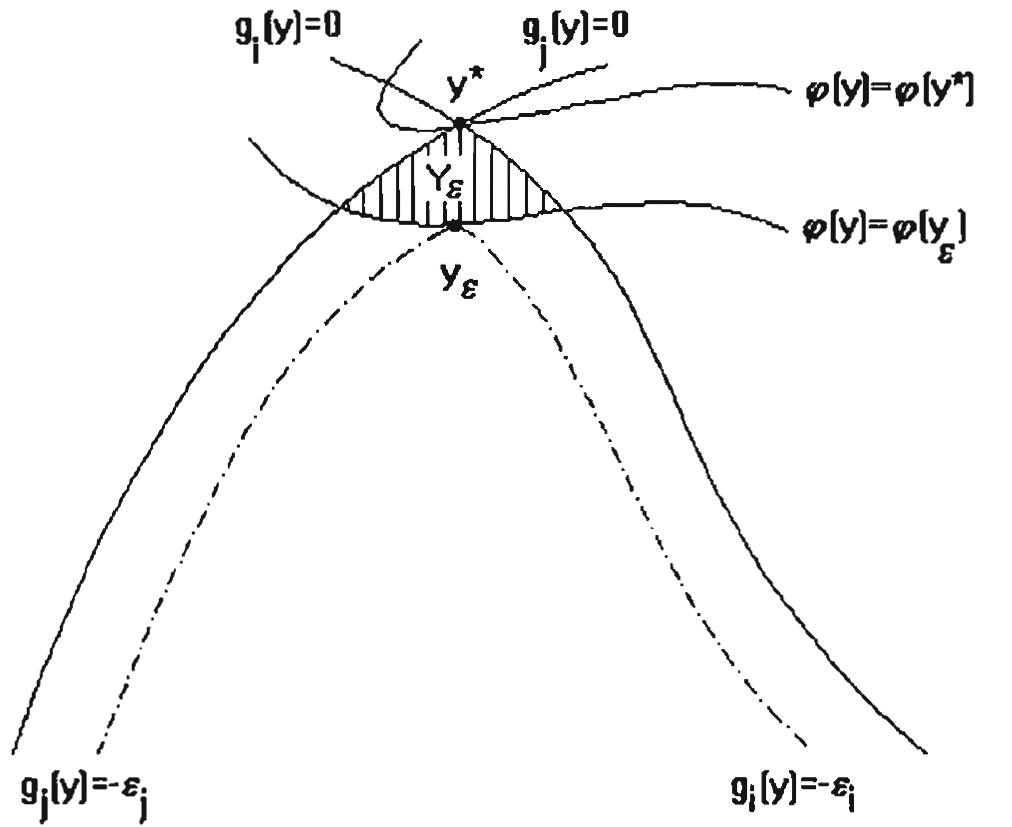
\includegraphics[width=0.7\linewidth]{figures/6_1.png}
\caption{$\epsilon$-reserved solution}
\label{6_fig_1}     
\end{figure}

The existence of the $\epsilon$-reserved solution of problem (\ref{6_problem}) can be interpreted as an analog of the regularity conditions in the classical problems of nonlinear programming. It should be noted also the applied importance of this condition. Even if the exact solution $y^\ast$ is known, its practical realization is possible as some approximation of $y^\ast$ only. Therefore, it is important that there exist the points from the feasible domain $Q$ close to $y^\ast$ (with respect to the coordinates and values). The existence of the $\epsilon$-reserved solution guarantees the existence of such points. In this case, the domain $Y_\epsilon$ can play a role of the set of suitable approximations.

Prior to going to the detailed description of the Peano curves and of the algorithm, let us consider some properties of reduced problem (\ref{6_problem_1}), which are absent in the pure one-dimensional case. First, as it has been already mentioned above, the functions $g_j(y(x)), \; 1 \leq j \leq m+1,$ are not Lipschitzian. They satisfy H\"older condition. Consequently, all the interval lengths in the search algorithm rules have to be replaced by the lengths in the metric
\[
\rho (x',x'') = \left(\left|x'-x''\right|\right)^{1/N}, \; x',x'' \in [0,1].
\]
Second, in general, sets (\ref{6_Q}) being the inverse images of the essentially non-cubic $N$-dimensional subsets with the nonlinear boundaries $g_j(y)=0, \; y \in D, \; 1\leq j \leq m,$ are not the finite unions of $x$-intercepts. Consequently, taking into account the $\epsilon$-reserved solutions plays a significantly more important role for the convergence in the reduced univariate problem (\ref{6_problem_1}) than in the pure one-dimensional case.

The issues of the numerical construction of the Peano-type space filling curves and the corresponding theory are considered in details in \cite{6_Butz,6_Sagan,6_Strongin2000,6_Strongin2013}. Here we will describe the basic steps of constructing a curve mapping a unit interval of the real axis $[0,1]$ onto a hypercube  
\[
D=\left\{y\in R^N: -2^{-1}\leq y_i \leq 2^{-1}, 1\leq i \leq N \right\}.
\]

\begin{enumerate}
	\item 
A hypercube $D$ with the unit edge length is divided by the coordinate hyperplanes into $2^N$ hypercubes of the first partition (with the edge length equal to $1/2$), which are indexed by the numbers $z_1$ ranging from $0$ to $2^N-1$. Let us agree to designate the hypercube of the first partition with the index $z_1$ as $D(z_1)$.

Next, each hypercube of the first partition is also divided into $2^N$ hypercubes of the second partition (with the edge length equal to $1/4$) by the hyperplanes parallel to the coordinate axes and crossing the middles of the hypercube edges orthogonal to these hyperplanes. The hypercubes of the second partition  included in the hypercube $D(z_1)$ are indexed by the numbers $z_2$ ranging from $0$ to $2^N-1$. The hypercube of the second partition  with the index $z_2$ from  $D(z_1)$ is denoted as $D(z_1, z_2)$. The case of $N=2$ is presented in Fig.~\ref{6_fig_2} for $m=1$, $m=2$.

\begin{figure}
\begin{minipage}{0.5\linewidth}
\center{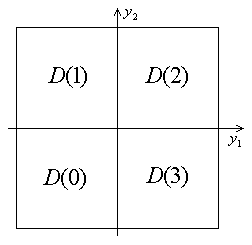
\includegraphics[width=0.9\linewidth]{figures/6_2a.png} \\ $m=1$}
\end{minipage}
\hfill
\begin{minipage}{0.5\linewidth}
\center{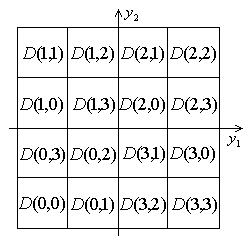
\includegraphics[width=0.9\linewidth]{figures/6_2b.png} \\ $m=2$}
\end{minipage}
\caption{The partition of an $N$-dimensional hypercube}
\label{6_fig_2}
\end{figure}

Continuing this process, one can construct the hypercubes of any $m$-th partition with the edge length equal to $(1/2)^m$, which are denoted as $D(z_1,...,z_m)$. It is obvious, that $D(z_1) \supset D(z_1,z_2) \supset ... \supset D(z_1,...,z_m)$ and $0 \leq z_j \leq 2^N-1$, \mbox{$1 \leq j \leq m$}.

\item
Now let us perform the division of the interval $[0,1]$ into $2^N$ equal parts, each of them also is divided into $2^N$ equal parts, etc. The elements of each partition are indexed from the left to the right by the numbers $z_j$ ranging from $0$ to \mbox{$2^N-1$} where $j$ is the index of subdivision. Let us denote the intervals of the $m$-th partition as $d(z_1,...,z_m)$ where, for example, $d(z_1,z_2)$ means the interval of the second partition with the index $z_2$ being a part of the interval $d(z_1)$ of the first partition with the index $z_1$.

One can note that  $d(z_1) \supset d(z_1,z_2) \supset ... \supset d(z_1,...,z_m)$ and the length of the interval $d(z_1,...,z_m)$ is equal to  $(1/2)^{mN}$. An interval $d(z_1,...,z_m)$ is supposed to include its left hand end. It contains its right hand boundary if and only if when $z_1=z_2=...=z_m=2^N-1$. The case of $N=2$ is presented in Fig.~\ref{6_fig_3} for $m=1$ and $m=2$.

\begin{figure}[t]
%\sidecaption[t]
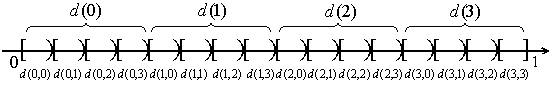
\includegraphics[width=0.9\linewidth]{figures/6_3.png}
\caption{Partition of a one-dimensional interval}
\label{6_fig_3}     
\end{figure}

\item
Assume that the point $y(x) \in D$ corresponding to the point $x \in [0,1]$ for any $m \geq $ belongs to the hypercube $D(z_1,...,z_m)$ if $x$ falls into the interval $d(z_1,...,z_m)$, i.e.,
\[
x \in d(z_1,...,z_m) \rightarrow y(x) \in D(z_1,...,z_m).
\]
The constructed correspondence  $y(x)$ is single-valued.
\item
In order to provide the continuity of the constructed correspondence, let us impose the following requirements on the indexing order of the hypercubes of each partition. Since $2^{mN}$ centers $y(z_1,...,z_m)$ of the hypercubes of the $m$-th partition $D(z_1,...,z_m)$ form a uniform orthogonal grid in the domain $D$ (the step of this grid with respect to any coordinate is equal to $2^{-m}$), one can introduce the following numeration of the grid nodes. Let us enumerate from the left to the right by index $i$ all subintervals of the $m$- 	th partition in the interval $[0,1]$, i.e.,
\[
d(z_1,...,z_m)=[x_i, x_{i+1}), \; 0 \leq i < 2^{mN}-1,
\]
were the left end of the $i$-th interval is denoted as $x_i$.

Assume the center of the hypercube $D(z_1,...,z_m)$ to have the same index $i$ as the interval $d(z_1,...,z_m)$ corresponding to this hypercube, i.e.,
\[
y_i = y(z_1,...,z_m), \; 0 \leq i < 2^{mN}-1.
\]
The centers $y_i$ and $y_{i+1}$ correspond to the adjacent hypercubes having a common facet. More details on the indexing of the hypercubes can be found in \cite{6_Strongin2013}.
\end{enumerate}

Let us consider the mapping  $l(x)$ of the interval $[0,1]$ into a hypercube $D$ defined by the expression 
\[
l(x)=y_i+(y_{i+1}-y_i)\frac{w(x)-x_i}{x_{i+1}-x_i}, \; x_i \leq w(x) \leq x_{i+1},
\]
\[
w(x)=x(1-2^{-mN}), \; 0 \leq x \leq 1.
\]
The image of any subinterval
\[
\left[x_i(1-2^{-mN})^{-1}, x_{i+1}(1-2^{-mN})^{-1}\right], \; 0 \leq i < 2^{mN}-1
\]
of the interval $[0,1]$ for the correspondence $l(x)$ is a linear segment connecting the nodes $y_i$ and $y_{i+1}$.

Thus, we have built a piecewise linear curve $l_m(x), 0 \leq x \leq 1,$ connecting the nodes $y_i, 0 \leq i< 2^{mN}-1,$ in the order of their indexing. This curve obtained numerically (\textit{the evolvent})  is an approximation of the theoretical Peano curve with the precision not worse than $2^{-m}$ with the respect to each coordinate (the parameter m is called\textit{ the density of the evolvent}). As an illustration, an image of the interval $[0,1]$ for the mapping $l_m(x)$ in the case $N=2, m=3$ is presented in Fig.~\ref{6_fig_4}. The grid nodes are marked with the dark circles. 

\begin{figure}[t]
%\sidecaption[t]
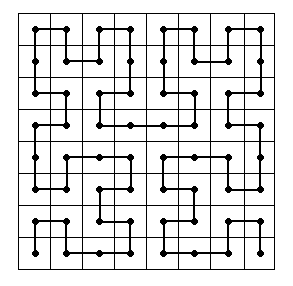
\includegraphics[width=0.5\linewidth]{figures/6_4.png}
\caption{A piecewise linear curve}
\label{6_fig_4}     
\end{figure}

\section{Multidimensional generalized global search algorithm}
The considered dimensionality reduction scheme associates a multidimensional problem with Lipschitz objective function and Lipschitz constraints with a one-dimensional problem, where the corresponding functions satisfy uniform H\"older condition (\ref{6_Holder}). As result, all lengths of the intervals appearing in the rules of the search algorithm should be replaced by the lengths in a new metrics, where the distance is defined by the expression
\[
\Delta_i = \left|x_i-x_{i-1}\right|^{1/N}.
\]
Also, in the reduction of the problem dimensionality by Peano curve  $y(x), 0 \leq x \leq 1,$ a trial at a point $x^k \in [0,1]$ executed at the $k$-th iteration of the algorithm will consist in the following sequence of operations.
\begin{itemize}
	\item Determine the image  $y^k=y(x^k)$ in accordance with the mapping  $y(x)$.
	\item Compute the values  $g_1(y^k),...,g_\nu(y^k)$, where the index $\nu \leq m$ are determined by the conditions
	\[
	g_j(y^k)\leq 0, \; 1 \leq j<\nu, \; g_\nu(y^k)>0, \; \nu \leq m.
	\]
	The occurrence of the first violation of the constraint terminates the trial at the point $y^k$. In the case, when the point $y^k$ is a feasible one, i.e., when $y(x^k) \in Q_{m+1}$, the trial includes the computation of the values of all functions of the problems and the index is accepted to be $\nu = m+1$. The pair of values
	\begin{equation}\label{6_trial_res}
	\nu = \nu(x^k), \; z^k = g_\nu(y(x^k))
	\end{equation}
	is a \textit{result of the trial} at the point $x^k$.
\end{itemize}

Thus, one can easily modify the initial one-dimensional algorithm and obtain on this base a multidimensional \textit{generalized index global search algorithm}, described below.

The first trial is executed at an arbitrary internal point $x^1 \in (0,1)$. The selection of the point $x^{k+1}, k \geq 1,$ of any next trial is determined by the following rules.

Rule 1. Renumber the points $x^1,...,x^k$ of the preceding trials by the
lower indices in ascending order of coordinate values, i.e.
\begin{equation}\label{6_trial_points}
0=x_0<x_1<\dots <x_k<x_{k+1}=1,
\end{equation}
and juxtapose to them the values $z_i=g_\nu(y(x_i)), \; \nu=\nu(x_i), \; 1 \leq i \leq k$, from (\ref{6_trial_res}) computed at these points. The points $x_0=0$ and
$x_{k+1}=1$ are introduced additionally for the convenience of further notations, while the values $z_0$ and
$z_{k+1}$ are not defined.

Rule 2. Classify the indices $i, \; 1 \leq i \leq k$, of the trial points (\ref{6_trial_points})
according to the number of the problem constraints fulfilled at these points by constructing the sets
\[
I_\nu =\left\{i:1 \leq i \leq k, \; \nu=\nu(x_i) \right\}, \; 1 \leq \nu \leq m+1,
\]
containing the numbers of all the points $x_i, \; 1 \leq i \leq k$, with
the same values of $\nu$. The end points $x_0=0$ and $x_{k+1}=1$ are
interpreted as the ones having indices equal to zero. An additional set $I_0=\left\{0,k+1\right\}$ corresponds to them.

Determine the maximum value of the index
\[
M=\max\left\{\nu(x_i), \; 1 \leq i \leq k \right \}.
\]

Rule 3. Compute the current lower estimates
\begin{equation}\label{6_mu}
\mu = \max\left\{ \frac{\left|z_i-z_j\right|}{ (x_i - x_j)^{1/N} }, \; i,j \in I_\nu, \; i>j \right\}
\end{equation}
for the unknown H{\"o}lder constants $K_\nu$ of the functions $g_\nu(y),1
\leq \nu \leq m+1$. If a set $I_\nu$ contains less than two elements, or
if $\mu_\nu$ from (\ref{6_mu}) is equal to zero, then assume $\mu_\nu=1$.

Rule 4. For all nonempty sets $I_\nu, \; 1 \leq \nu \leq m+1$, compute the
estimates
\[
z_\nu^\ast = \left\{
   \begin{array}{lr}
     -\epsilon_\nu, & \nu < M,\\
     \min\{ g_\nu(y(x_i)): i\in I_\nu \}, & \nu = M,
   \end{array}
\right.
 \]
where the vector $\epsilon_R = (\epsilon_1,...,\epsilon_m)$ is a predefined vector with the nonnegative components (\textit{the reserve vector}).

Rule 5. For each interval ($x_{i-1},x_i), \; 1 \leq i \leq k+1,$ compute
the \textit{characteristics} $R(i)$ :
\[
R(i)=2\Delta_i-4\frac{z_i-z_\nu^\ast}{r_\nu \mu_\nu}, \; \nu=\nu(x_i)>\nu(x_{i-1}),
\]
\begin{equation}%\label{eq:14}
R(i)=\Delta_i+\frac{(z_i-z_{i-1})^2}{r_\nu^2 \mu_\nu^2\Delta_i}-2\frac{z_i+z_{i-1}-2z_\nu^\ast}{r_\nu \mu_\nu}, \;  \nu=\nu(x_i)=\nu(x_{i-1}),
\end{equation}
\[
R(i)=2\Delta_i-4\frac{z_{i-1}-z_\nu^\ast}{r_\nu \mu_\nu}, \; \nu=\nu(x_{i-1})>\nu(x_i),
\]
where $\Delta_i=(x_i - x_{i-1})^{1/N}$. The values $r_\nu > 1, \; 1 \leq
\nu \leq m+1,$ are parameters of the algorithm. An appropriate selection
of $r_\nu$ allows to consider the product $r_\nu \mu_\nu$ as an estimate
of the H{\"o}lder constants $K_\nu, \; 1 \leq \nu \leq m+1$.

Rule 6. Find the interval $(x_{t-1},x_t)$ with the maximum characteristic
\begin{equation}\label{6_MaxR}
R(t)=\max{\left\{R(i): 1 \leq i \leq k+1\right\}}.
\end{equation}

Rule 7. Make the next trial at the midpoint of the interval
$(x_{t-1},x_t)$ if the indices of the points $x_{t-1}$ and $x_t$  are not
the same, i.e.,
\[
x^{k+1} = \frac{x_t + x_{t-1}}{2}, \; \nu(x_{t-1}) \neq \nu(x_t).
\]
Otherwise, make the trial at the point
\begin{equation}%\label{eq:142}
x^{k+1} = \frac{x_t+x_{t-1}}{2} - \frac{\mathrm{sign}(z_t-z_{t-1})}{2r_\nu}\left[\frac{\left|z_t-z_{t-1}\right|}{\mu_\nu}\right]^N, \; \nu=\nu(x_{t-1})=\nu(x_t).
\end{equation}

We may take as termination condition the inequality $\Delta_t \leq
\epsilon$, where $t$ is from (\ref{6_MaxR}) and $\epsilon>0$ is the
predefined accuracy.

\textbf{The algorithm convergence conditions.} These conditions are a special case of the convergence theorem which will be proved in Subsection 6.3 for the parallel algorithm with a single curve on a single processor.

\begin{example} \label{6_example1}
As an illustration, let us consider the problem of minimization of the function
\begin{align*}
 \varphi(y_1,y_2) = &-1.5y_1^2\exp(1-y_1^2-20.25(y_1-y_2)^2)- \\
				            &-(0.5(y_1-1)(y_2-1))^4\exp(2-(0.5(y_1-1))^4-(y_2-1)^4)
\end{align*}
within the domain $0 \leq y_1\leq 4,\ -1\leq y_2\leq 3$, with the constraints 
\begin{align*}
g_1(y_1,y_2)&=0.01((y_1-2.2)^2+(y_2-1.2)^2-2.25)\leq 0,\\
g_2(y_1,y_2)&=100(1-(y_1-2)^2/1.44-(0.5y_2)^2)\leq 0,\\
g_3(y_1,y_2)&=10(y_2-1.5-1.5\sin(6.283(y_1-1.75)))\leq 0.
\end{align*}

Fig.~\ref{6_fig_5} shows the square search domain and the points of $1098$ trials obtained by the index method with the following parameters: the reliability parameters $r_1=...=r_4=2$, the accuracy $\epsilon = 10^{-3}$, the evolvent density $m=12$.
\begin{figure}[t]
%\sidecaption[t]
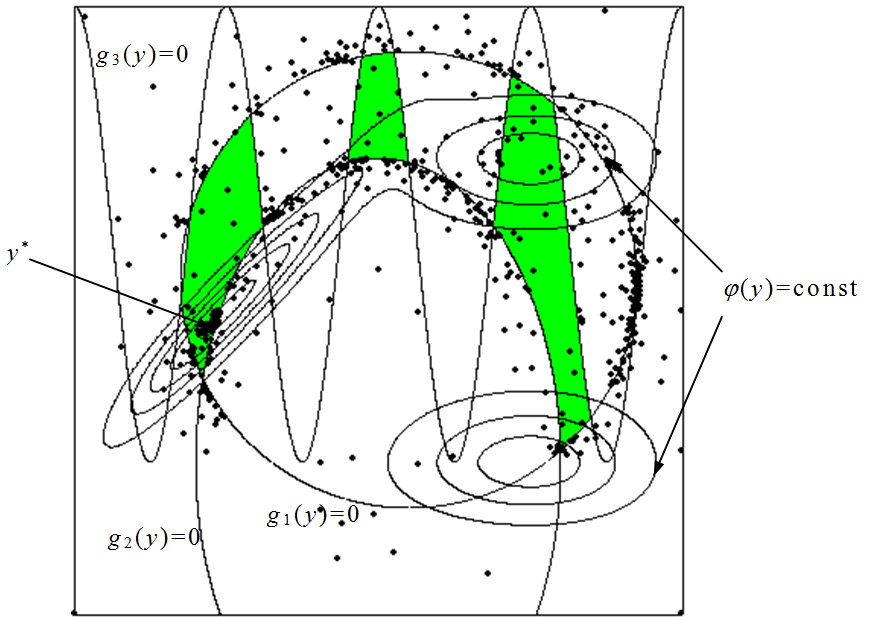
\includegraphics[width=0.8\linewidth]{figures/6_5.png}
\caption{The results of solving the test problem}
\label{6_fig_5}     
\end{figure}

\end{example}

Note that in applied problems, estimating the values of the constraints and of the objective functions very often requires considerable computation resources. The results of the experiments confirm the efficiency of the index scheme of the accounting for the constraints since the values of the functions $g_1,\ g_2,\ g_3,\ \varphi = g_4$ were computed $k_1=1098,\ k_2=623,\ k_3=392,$ and $k_4=152$ times, respectively. If the search of the solution were conducted on a uniform grid, in order to achieve the same accuracy $\epsilon=10^{-3}$ $k_1=1.6\cdot 10^7,\ k_2=7 \cdot 10^6,\ k_3=3\cdot 10^6,$ and $k_4=1.4 \cdot 10^6$ computations of the values of the functions $g_1,\ g_2,\ g_3,\ \varphi = g_4$, respectively, would be necessary.

\section{Parallel multidimensional multiextremal methods based on multiple Peano curves}

\subsection{Application of multiple mappings}\label{6_section_shift}

The reduction of the multidimensional problems to the one-dimensional ones using the Peano curves has such important properties as the continuity and the uniform boundedness of the function differences for limited variation of argument. However, a partial loss of information on the nearness of the points in the multidimensional space takes place since a point $x \in [0,1]$ has the left and the right neighbors only while the corresponding point $y(x) \in D \subset R^N$ has the neighbors in $2N$ directions. As a result, when using the mappings like Peano curve the images $y',\ y'',$ which are close to each other in the $N$-dimensional space can correspond to the preimages $x',\ x'',$ which can be far away from each other in the interval $[0,1]$. This property results in the excess computations since several limit points $x',\ x''$ of the trial sequence generated by the index method in the interval $[0,1]$ can correspond to a single limit point $y$ in the $N$-dimensional space.

One of the possible ways to overcome this disadvantage consists in using the multiple mappings
\begin{equation}%\label{eq:142}
Y_L(x)=\left\{y^0(x),\ y^1(x),...,\ y^L(x)\right\}
\end{equation}
instead of single Peano curve $y(x)$ (see \cite{6_Strongin1991,6_Strongin1992,6_Strongin2000}).

Let us consider a family of the hypercubes 
\begin{equation}\label{6_hypercubes}
D_l= \left\{y \in R^N: -2^{-1} \leq y_i+2^{-l} \leq 3 \cdot 2^{-1},\ 1\leq i\leq N\right\},\ 0 \leq l \leq L,
\end{equation}
where the hypercube $D_{l+1}$ is obtained by the translation of the hypercube $D_l$ along the main diagonal with displacement equal to $2^{-l}$ in each coordinate. In Fig.~\ref{6_fig_6} the hypercubes $D_0,...,D_3$ for the case $N=2,\ L=3$ are presented.

\begin{figure}[t]
%\sidecaption[t]
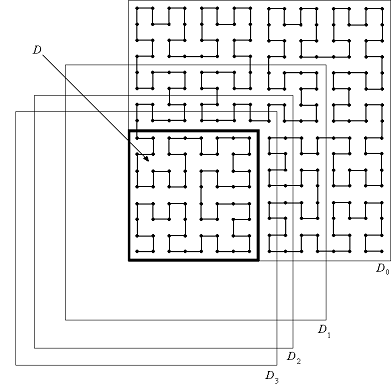
\includegraphics[width=0.7\linewidth]{figures/6_6.png}
\caption{Multiple mappings}
\label{6_fig_6}     
\end{figure}

Let us assume that the evolvent $y^0(x)$  maps the interval $[0,1]$ onto the hypercube $D_0$ from (\ref{6_hypercubes}), i.e.,
\[
D_0 = \left\{y^0(x) : x \in [0,1]\right\}.
\]
Then, the evolvents $y^l(x)=\left\{y_1^l(x),...,y_N^l(x)\right\}$, the coordinates of which are defined by the conditions 
\[
y_i^l(x)=y_i^{l-1}(x)+2^{-l},\ 1\leq i\leq N, \ 1\leq l\leq L,
\]
map the interval $[0,1]$ onto the corresponding hypercubes $D_l,\ 1\leq l \leq L$. In Fig.~\ref{6_fig_6} the image of the interval $[0,1]$ obtained by the curve $y^0(x),\ x\in [0,1],$ is shown as the broken line. Since the hypercube $D$ from (\ref{6_D}) is included in the common part of the family of hypercubes (\ref{6_hypercubes}) (the boundaries of hypercube $D$ are highlighted in Fig.~\ref{6_fig_6}), having introduced an additional constraint function
\begin{equation}\label{6_g0}
g_0(y)=\max\left\{\left|y_i\right| - 2^{-1}:\ 1\leq i\leq N\right\},
\end{equation}
one can present the initial hypercube $D$ in the form
\[
D=\left\{y^l(x):\; x\in [0,1],\ g_0(y^l(x))\leq 0 \right\},\ 0\leq l \leq L,
\]
i.e., $g_0(y) \leq 0$ if $y\in D$ and $g_0(y)>0$ otherwise. Consequently, any point $y \in D$ has its own preimage $x^l \in [0,1]$ for each mapping $y^l(x),\ 0\leq l\leq L$.

Thus, each evolvent $y^l(x),\ 0\leq l \leq L,$ generates its own problem of the type (\ref{6_problem_1}) featured by its own extended (in comparison with $D$) search domain $D_l$ and the additional constraint with the left hand part from (\ref{6_g0})
\begin{equation}\label{6_problem_l} 
\min{\left\{\varphi(y^l(x)):x\in [0,1], \; g_j(y^l(x))\leq 0, \; 0 \leq j \leq m\right\}}, \ 0 \leq l \leq L.
\end{equation} 

The problems (\ref{6_problem_l}) correspond to the domains $Q_0^l=[0,1]$ and $Q_{j+1}^l, 0 \leq j \leq m,$ defined by the expression 
\[
Q_{j+1}^l = \left\{x \in Q_j^l:g_j(y^l(x))\leq 0\right\},\ 0\leq j\leq m,
\]
for the corresponding evolvents $y^l(x)$. The application of a multiple mapping defines the following relation for the nearness in the multidimensional search domain and in the one-dimensional one.

\begin{theorem}
Let a point $y^\ast$ from the domain $D$ be contained in the line segment with the end-points $y',y'' \in D$ meeting the requirements 
\[
\left|y'_j - y''_j\right|\leq 2^{-p},\ y'_i=y''_i=y^\ast_i, \ 1\leq i \leq N,\ i \neq j,
\]
where $p$ is an integer  and $1\leq p \leq L$, i.e., the line segment is collinear with the $j$-th axis in $R^N$. Then, there exist at least one mapping $y^l(x),\ 0\leq l\leq L$, and the preimages $x^\ast,\; x',\; x''\in [0,1]$ such that
\[
y^\ast = y^l(x^\ast),\ y'=y^l(x'),\ y'' = y^l(x'')
\]
and
\[
\max \left\{ \left|x'-x^\ast\right|,\; \left|x''-x^\ast\right|,\; \left|x'-x''\right|\right\} \leq 2^{-pN}.
\]
\end{theorem}
\begin{proof}
Proof of this theorem is given in \cite{6_Strongin2000}.
\qed
\end{proof}

The conditions of the theorem single out a specific vicinity of the point $y^\ast$. This vicinity includes only the points, which can be obtained by the shift of $y^\ast$ parallel to one of the coordinate axes with a displacement not more than $2^{-p}$. By changing  $j,\ 1\leq j\leq N,$ in the theorem conditions it is possible to obtain the neighbours in any $N$ coordinate directions. According to the statement, the closeness of the points in the $N$-dimensional space in a particular direction will be reflected by the closeness of their preimages in one of the univariate problems. The information on the closeness of the points results, first, in more precise estimate of Lipschitz constants and, second, in the increase of the characteristics of the intervals, the images of the end points of which are close to each other in the $N$-dimensional space.

\subsection{Organization of the parallel computations}

Using the multiple mappings allows solving initial problem (\ref{6_problem}) by parallel solving $L+1$ problems of the type (\ref{6_problem_l}) on a set of intervals $[0,1]$ by the index method. Each univariate problem is solved on a separate processor. The results of trial at the point $x^k$ obtained on a particular processor for the problem being solved by this processor are interpreted as the results of the trials in the rest problems (in the corresponding points $x^{k0},\ x^{k1},...,x^{kL}$). In this approach, a trial at the point $x^k \in [0,1]$ executed in the framework of the $s$-th problem, consists in the following sequence of operations.
\begin{enumerate}
	\item Determine the image $y^k=y^s(x^k)$ at the mapping  $y^s(x)$.
	\item Compute the value $g_0(y^k)$. If $g_0(y^k) \leq 0$, i.e., if $y^k \in D$, then inform the rest processors on the start of the trial execution at the point $y^k$ (\textit{the blocking} of the point $y^k$).
	\item Compute the values $g_1(y^k),...,g_\nu(y^k),$ where the index $\nu \leq m$ are determined by the conditions
	\[
	g_j(y^k)\leq 0,\ 1\leq j< \nu,\ g_\nu(y^k) > 0,\ \nu \leq m.
	\]
	The occurrence of the first violation of any constraint terminates the trial at the point $y^k$. In the case when $y^k$ is a feasible one, i.e., when $y^s(x^k) \in Q_{m+1}$, the trial includes the computation of all functions of the problem. In this situation the index is set to $\nu = m+1$. The triplet
	\begin{equation}\label{6_triplet} 
	y^s(x^k),\ \nu = \nu(x^k),\ z^k=g_\nu(y^s(x^k))
	\end{equation}
	is  \textit{the trial result} at the point $x^k$.
	\item If $\nu (x^k)>0$, i.e., if $y^k \in D$, then determine the preimages $x^{kl} \in [0,1],\; 0\leq l \leq L,$ of the point $y^k$ and interpret the trial executed at the point $y^k \in D$ as the execution of the trials in the $L+1$ points 
	\[
	x^{k0},\ x^{k1},...,\ x^{kL}
	\]
	with the same result 
	\[
	\nu(x^{k0})=\nu(x^{k1})=...=\nu(x^{kL})=\nu(x^k),	
	\]
	\[
	g_\nu(y^0(x^{k0}))=g_\nu(y^1(x^{k1}))=...=g_\nu(y^L(x^{kL}))=z^k	
	\]
	and inform the rest processors on the results of the trial at the point $y^k$.	
	In the case if $\nu (x^k)=0$, i.e., if $y^k \notin D$, the trial result is related only to the $s$-th problem.	
\end{enumerate}

Each processor has its own copy of the software realizing the computations of the problem functions and the decision rule of the algorithm. For the organization of the interactions among the processors, $L+1$ queues are created on each processor, where the processors store the information on the iterations executed in the form of the triples (\ref{6_triplet}). Moreover, the index of the blocked point is assumed to be equal to $–1$; the function value at this point is undefined. The links among the processors by means of the queues $Q_{ls}$, where $l,\; 0\leq l \leq L,$ is the number of the transmitting processor and $s,\; 0 \leq s \leq L,$ is the index of the receiving processor, are illustrated in Fig.~\ref{6_fig_7}.

\begin{figure}[t]
%\sidecaption[t]
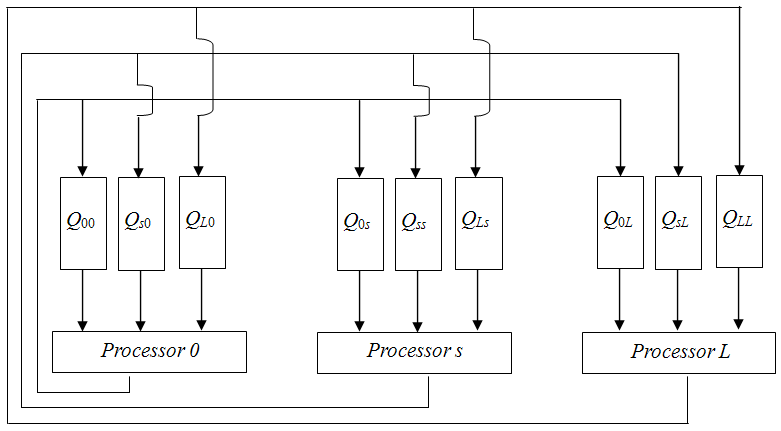
\includegraphics[width=0.8\linewidth]{figures/6_7.png}
\caption{The links among the processors }
\label{6_fig_7}     
\end{figure}

The proposed scheme does not include any managing processor that increases the reliability of the computations executed. The decision rules for the proposed parallel algorithm, in general, are the same as the rules of the sequential algorithm (except the method of the trial execution). However, in the purposes of deeper understanding of the subject, the scheme is presented here in full.

The algorithm for the selection of the iteration points is the same for all processors. The starting iteration is executed at a predefined point $x^1 \in (0,1)$ (the starting points for all processors are different). The selection of any next iteration point $x^{q+1}$, $q \geq 1$, is determined by the following rules.

Rule 1. Extract from all queues associated with $l$-th processor the results stored for this processor including the set of the iteration points $Y_q=\left\{y^{qi}:1 \leq i \leq s_q\right\}$,  the indices and the function values from (\ref{6_triplet}) computed at these points; determine the set $X_q={x^qi:1\leq i \leq s_q}$ of preimages of the points from the set $Y_q$ for the evolvent $y^l(x)$.

Rule 2. Renumber the points of the set of iterations
\[
\{x_1\} \cup X_1 \cup ... \cup X_q
\]
by the subscripts in increasing order of the coordinate
\begin{equation}\label{6_points_x} 
	0=x_0<x_1< \dots <x_k<x_{k+1}=1,
\end{equation}
where $k=1+s_1+\dots+s_q$, and juxtapose to them the values $z_i=g_\nu(x_i)$, $\nu = \nu(x_i)$, $1 \leq i \leq k$, computed at these points. The index of the blocked point $x_i$ (i.e., of the point, where other trial has been already started by other processor) is set to $–1$, i.e., $\nu(x_i)=-1$ and the value $z_i$ is undefined. The points $x_0,\ x_{k+1}$ are introduced additionally for the convenience of further presentation, the indices of these points are set to $-2$, i.e., $\nu(x_0)=\nu(x_{k+1})=-2$ and the values $z_0,\ z_{k+1}$ are undefined.

Rule 3. Perform the classification of the subscripts $i,\ 1 \leq i \leq k,$ of the points from (\ref{6_points_x}) in accordance with  the number of problem constraints fulfilled in these points by constructing the sets
\[
I_{-2} = \{0, k+1\},
\]
\[
I_{-1} = \{i: 1 \leq i \leq k,\ \nu(x_i)=-1\},
\]
\[
I_{\nu} = \{i: 1 \leq i \leq k,\ \nu(x_i)=\nu\},\ 0 \leq \nu \leq m+1,
\]
including the indices of all points $x_i,\ 1 \leq i \leq k,$ with the same indices equal to $\nu$. 
Determine the maximum value of the index
\[
M=\max\left\{\nu(x_i), \; 1 \leq i \leq k \right \}.
\]

Rule 3. Compute the current lower estimates
\begin{equation}\label{6_mu_par}
\mu = \max\left\{ \frac{\left|z_i-z_j\right|}{ (x_i - x_j)^{1/N} }, \; i,j \in I_\nu, \; i>j \right\}
\end{equation}
for the unknown H{\"o}lder constants $K_\nu$ of the functions $g_\nu(y),1
\leq \nu \leq m+1$. If a set $I_\nu$ contains less than two elements, or
if $\mu_\nu$ from (\ref{6_mu_par}) is equal to zero, then assume $\mu_\nu=1$.

Rule 4. For all nonempty sets $I_\nu, \; 1 \leq \nu \leq m+1$, compute the
values
\begin{equation}\label{6_z_nu}
z_\nu^\ast = \left\{
   \begin{array}{lr}
     -\epsilon_\nu, & \nu < M,\\
     \min\{ g_\nu(y(x_i)): i\in I_\nu \}, & \nu = M,
   \end{array}
\right.
\end{equation}
where the vector $\epsilon_R = (\epsilon_1,...,\epsilon_m)$ is a predefined vector with the nonnegative components (\textit{the reserve vector}).

Rule 5. For each interval ($x_{i-1},x_i), \; 1 \leq i \leq k+1,$ compute
the \textit{characteristics} $R(i)$ :
\[
R(i)=2\Delta_i-4\frac{z_i-z_\nu^\ast}{r_\nu \mu_\nu}, \; \nu=\nu(x_i)>\nu(x_{i-1}),
\]
\begin{equation}\label{6_R_par}
R(i)=\Delta_i+\frac{(z_i-z_{i-1})^2}{r_\nu^2 \mu_\nu^2\Delta_i}-2\frac{z_i+z_{i-1}-2z_\nu^\ast}{r_\nu \mu_\nu}, \;  \nu=\nu(x_i)=\nu(x_{i-1}),
\end{equation}
\[
R(i)=2\Delta_i-4\frac{z_{i-1}-z_\nu^\ast}{r_\nu \mu_\nu}, \; \nu=\nu(x_{i-1})>\nu(x_i),
\]
\[
\Delta_i=(x_i - x_{i-1})^{1/N}
\]
The values $r_\nu > 1, \; 1 \leq \nu \leq m+1,$ are parameters of the algorithm. 

Rule 6. Find the interval $(x_{t-1},x_t)$ with the maximum characteristic
\begin{equation}\label{6_MaxR_par}
R(t)=\max{\left\{R(i): 1 \leq i \leq k+1\right\}}.
\end{equation}

Rule 7. Make the next trial at the midpoint of the interval
$(x_{t-1},x_t)$ if the indices of the points $x_{t-1}$ and $x_t$  are not
the same, i.e.,
\begin{equation}\label{6_x_new_par_1}
x^{q+1} = \frac{x_t + x_{t-1}}{2}, \; \nu(x_{t-1}) \neq \nu(x_t).
\end{equation}
Otherwise, make the trial at the point
\begin{equation}\label{6_x_new_par_2}
x^{q+1} = \frac{x_t+x_{t-1}}{2} - \frac{\mathrm{sign}(z_t-z_{t-1})}{2r_\nu}\left[\frac{\left|z_t-z_{t-1}\right|}{\mu_\nu}\right]^N, \; \nu=\nu(x_{t-1})=\nu(x_t).
\end{equation}
If $\nu(x^{q+1})=0$, i.e. $y^{q+1} \notin D$, then store the trial results only in queue assigned to the current processor itself. If $\nu(x^{q+1})>0$, i.e. $y^{q+1} \in D$, then store the trial results in all queues assigned to the current processor. 

The stopping condition will terminate the search when the inequality
\[
\Delta_t \leq \epsilon
\]
holds, where $t$ is from (\ref{6_MaxR_par}) and $\epsilon > 0$ is a given search accuracy.

\subsection{The convergence conditions for the algorithm}

The sufficient convergence conditions for the considered parallel algorithm can be formulated in the following form.
\begin{theorem}\label{6_theorem}
Assume that the following conditions are satisfied.

\begin{enumerate}
	\item Problem (\ref{6_problem}) has an $\epsilon$-reserved solution $y_\epsilon$ from (\ref{6_eps_r}).
	\item Functions $g_j(y),\; 1\leq j\leq m+1,$ admit Lipschitzian (with the constants $L_j$) extensions $G_j(y)$ over the whole feasible domain $D$ from (\ref{6_D}), i.e.,
	\begin{equation}\label{6_lip_ext}
	g_j(y(x))=G_j(y(x)),\ x\in Q_j,\ 1\leq j\leq m+1,
	\end{equation}
	where the sets $Q_j$ are from (\ref{6_Q}) and $y(x)$ is the curve from (\ref{6_problem_1}).	
	\item The parameters of the method $\epsilon_\nu,\ 1\leq \nu \leq m,$ used in the rule (\ref{6_z_nu}) are the corresponding components of the reserve vector $\epsilon_R$ from (\ref{6_eps_r}).
	\item For sufficiently large iteration number $q$  the values $\mu_\nu$ from (\ref{6_mu_par}) satisfy the inequalities 
	\begin{equation}\label{6_inequalities}
	r_\nu\mu_\nu > 2^{3-1/N}L_\nu \sqrt{N+3},\ 1\leq \nu \leq m+1,	
	\end{equation}
	at least for one processor.
\end{enumerate}
Then, any limit point $\overline{y}$  of the sequence of the trials ${y^k}$ generated by the index algorithm for problem (\ref{6_problem}) belongs to the set $Y_\epsilon$ form (\ref{6_eps_solution}) and satisfies the conditions
	\begin{equation}\label{6_conditions}
	\varphi(\overline{y})=\inf \left\{\varphi(y^k):g_j(y^k)\leq 0, \; 1\leq j\leq m,\ k=1,2,\dots \right\}\leq \varphi(y_\epsilon).	
	\end{equation}
\end{theorem}
Prior to begin the proof of the theorem let us formulate and prove several auxiliary statements.
\begin{lemma}
Assume that the theorem conditions are satisfied. Then, for each limit point $\overline{y}$ of the sequence $\{y^k\}$ there exists an infinite sequence of the intervals 
	\begin{equation}\label{6_intervals}
	\{ \left( x_{t-1}, x_t\right): t=t(q^p), p=1,2,...	\},
	\end{equation}
	satisfying the conditions 
	\[
	\overline{x} = \bigcap_{p=1}^\infty\left[x_{t-1},x_t\right],
	\]
	\begin{equation}\label{6_limdelta}
	\lim_{p\rightarrow\infty}{\Delta_t} = 0,
	\end{equation}
	\begin{equation}\label{6_Rg0}
	R(t(q^p))>0, p=1,2,...,
	\end{equation}
	\begin{equation}\label{6_limR}
	\lim_{p\rightarrow\infty} R(t(q^p))=0,
	\end{equation}
where $q^1<q^2<...$; $R(t)$, $\Delta_t$ and $t$ are from the rules (\ref{6_R_par}), (\ref{6_MaxR_par}) correspondingly.
\end{lemma}
\begin{proof}
Since $\overline{y}$ is a limit point, there should exist such index $l,\ 0\leq l \leq L,$ that the $l$-th processor generates a sequence of the points $x^{q^l}$  converging to the preimage $\overline{x}^l$ of the point $\overline{y} = y^l(\overline{x}^l)$ . Consequently, there exists a sequence of the trial numbers $q^1,q^2,...,$ satisfying the conditions 
	\begin{equation}\label{6_xl}
	\overline{x}^l \in \left[x_{t-1},x_t\right],\ t=t(q),\ q\in \{ q^p \},\ p=1,2, ...
	\end{equation}
These conditions reflect the fact that the point of the $(q+1)$-th trial executed on the $l$-th processor falls into the interval $[x_{t-1},x_t]$ including the point $\overline{x}^l$ at the step $q$, i.e., $t=t(q)$.

It follows from (\ref{6_mu_par}), (\ref{6_x_new_par_1}), (\ref{6_x_new_par_2}),  and from condition (\ref{6_xl}) that
	\begin{equation}\label{6_len}
	\max\left\{x_t-x^{q^l},x^{q^l}-x_{t-1}\right\}\leq \gamma (x_t-x_{t-1}),
	\end{equation}
where $\gamma = (r+1)/2r < 1$, $r = \min \{ r_\nu : 1\leq\nu\leq m+1 \} >1$. Then, property (\ref{6_limdelta}) is a consequence of inequality (\ref{6_len}).

At every step $k \geq 1$ there exists an interval $(x_{i-1},x_i): i=i(k)$, at one of the ends of which  the value $z_M^\ast$ is reached, where $M$ is the largest index value. If $\nu (x_{i-1}) \neq \nu(x_i)$, according to rules (\ref{6_R_par}), $R(i)=2\Delta_i > 0$. In the case, when $\nu(x_{i-1})=\nu(x_i)=M$ the estimate 
\[
z_i+z_{i-1}-2z_M^\ast \leq \mu_M\Delta_i
\]
follows from (\ref{6_mu_par}). This estimate in combination with (\ref{6_R_par}) gives the inequality $R(i)=(1-r^{-1})\Delta_i>0$. Thus, at any search step $k\geq 1$ an interval with a strictly positive characteristic exists. Hence, taking into account (\ref{6_MaxR_par}) one can conclude that the intervals from system (\ref{6_intervals}) should have positive characteristic as well since they undergo partitioning by the trial points falling into these intervals, i.e., conditions (\ref{6_Rg0}) hold.

It follows from the selection rules for the values $z_\nu^\ast$ that
\[
z_j = g_\nu(x_j)\geq z_\nu^\ast,\ \nu=\nu(x_j),\ 1\leq j\leq k.
\]
Then, from the rules for the computation of the characteristics (\ref{6_R_par}) taking into account conditions (\ref{6_lip_ext}) and inequality (\ref{6_Rg0}) one can derive out the truth of (\ref{6_limR}).
\end{proof}

\begin{lemma} \label{6_lemma2}
(on the existence of a feasible point). 
Assume the conditions of theorem are satisfied. Then, there exists such number of trial $h \geq 1$, for which 
	\begin{equation}\label{6_fis_point}
	\nu(x^h)=m+1.
	\end{equation}
\end{lemma}
\begin{proof}
According to definition (\ref{6_eps_r}), the point $y_\epsilon$ is an internal point of a feasible domain. Consequently, for any mapping $y^l(x),\; 0\leq l \leq L,$ there exists a hypercube $D(m)$ of the $m$-th partitioning belonging to a feasible domain and including the $\epsilon$-reserved solution $y_\epsilon$. It means that there exists also a preimage interval $d(m)$ for the hypercube $D(m)$ and this interval includes the preimage $x_\epsilon$ of the point $y_\epsilon$, i.e., $y_\epsilon=y^l(x_\epsilon)$. At any search step $q>1$ there exists an interval $[x_{j-1},x_j],\; j=j(q),$ including the point $x_\epsilon$.

It follows from H\"older properties (\ref{6_Holder}) of the functions and from condition (\ref{6_lip_ext}) of the theorem that
	\begin{equation}\label{6_39}
	z_j=g_\nu(y^l(x_j))\leq g_\nu(y^l(x_\epsilon))+2L_\nu \sqrt{N+3}(x_j - x_\epsilon)^{1/N},\ \nu=\nu(x_j),
	\end{equation}
	\begin{equation}\label{6_40}
	z_{j-1}=g_\nu(y^l(x_{j-1}))\leq g_\nu(y^l(x_\epsilon))+2L_\nu \sqrt{N+3}(x_\epsilon -x_{j-1})^{1/N},\ \nu=\nu(x_{j-1}).
	\end{equation}
Moreover, it follows from condition (\ref{6_eps_r}) that
	\begin{equation}\label{6_41}
	g_\nu(y(x_\epsilon))\leq -\epsilon_\nu,\ 1\leq \nu \leq m.
	\end{equation}
If condition (\ref{6_fis_point}) is not satisfied at any of the search steps, then
\[
\nu = \max \{ \nu(x_{j-1}),\nu(x_j) \} \leq m,
\]
and it follows from conditions (\ref{6_R_par}), (\ref{6_inequalities}), and (\ref{6_39})--(\ref{6_41}) that at large enough $q$
\[
R(j(q)) \geq \Delta_j \left(1-\frac{4L_\nu\sqrt{N+3}}{r_\nu\mu_\nu}\right) + 4\frac{z_\nu^\ast+\epsilon_\nu}{r_\nu\mu_\nu}>0, \ \nu(x_{j-1})=\nu(x_j),
\]
\[
R(j(q)) \geq 2\Delta_j \left(1-\frac{2L_\nu\sqrt{N+3}}{r_\nu\mu_\nu}\right) + 4\frac{z_\nu^\ast+\epsilon_\nu}{r_\nu\mu_\nu}>0, \ \nu(x_{j-1}) \neq \nu(x_j).
\]

From these inequalities, from limit (\ref{6_limR}) as well as from rule (\ref{6_MaxR_par}) a necessity to execute the trials in the considered interval $[x_{j-1},x_j]$ at some search step follows, that results in its splitting into two subintervals. At least one of these includes the point $x_\epsilon$. The repetition of this process for $q\rightarrow \infty$ generates an infinite sequence of the subintervals collapses to the point $x_\epsilon$. It has been shown in the beginning of the proof of this lemma that there exists an interval $d(m)$ including the point $x_\epsilon$ and that all points of this interval are the internal points of a feasible domain, i.e., their indices are equal to $m+1$. Consequently, the interval $[x_{j-1},x_j]$ from the sequence of those collapsing to $x_\epsilon$ will belong to the interval $d(m)$. This proves the truth of (\ref{6_fis_point}).
\end{proof}

\begin{lemma} (on the feasibility of any limit point).
Any limit point $\overline{y}=y^l(\overline{x}^l)$  of the trial sequence $\{y^k\}$ is feasible, i.e., 
	\begin{equation}\label{6_rho}
	\nu(\overline{x}^l)=m+1.
	\end{equation}
\end{lemma} 
\begin{proof}
Let us assume that the limit point $\overline{y}$ is not feasible, i.e. that there exists such integer $\nu \geq 1$ that
\[
g_i(y(\overline{x}^l))\leq 0,\ 1\leq i\leq \nu - 1,\ g_\nu(y(\overline{x}^l))>0.
\]
Then, the point $\overline{y}$ has a vicinity $U_\rho(\overline{y})$ of the radius $\rho = \epsilon_\nu/2L_\nu$ such that all points of this vicinity satisfy the condition
	\begin{equation}\label{6_lim_fis_point}
	g_\nu(y) > -\epsilon_\nu/2, \ y \in U_\rho(\overline{y}).
	\end{equation}

If an integer number $M$ satisfies the inequality $2^{-M\sqrt{N}}<\rho$, there exists a subcube $D(M)$ including the point  $\overline{y}$. If $\overline{y}$ is an internal point of $D(M)$ then the preimage of this subcube $d(M)$ includes all preimages of the point $\overline{y}$. Consequently, $\overline{x}$ is an internal point of $d(M)$. 
If $\overline{y}$ is a corner of the subcube $D(M)$, there exists $2^N$ subcubes of the $M$-th  partitioning in $U_\rho(\overline{y})$, and their preimages include all preimages of the point $\overline{y}$ . 
It means that $\overline{x}^l$  belongs to one of the preimages. Let us denote this interval as  $d'(M)$. If $\overline{x}^l$ is an end point of $d'(M)$, this point is an end point of another interval $d''(M)$ as well. 
Consequently, the union $d'(M) \cup d''(M)$ includes $\overline{x}^l$ as an internal point. 
Thus, in any case there exists an interval $[\alpha,\beta] \subset [0,1] $ including $\overline{x}^l$ as an internal point and the images $y=y(x)$ of all points of the interval $(\alpha,\beta)$ satisfy condition (\ref{6_lim_fis_point}).

Since  $\overline{x}^l$  is a limit point, the intervals from the sequence $[x_{t-1},x_t],\ t=t(q)$, collapsing to this point should satisfy the condition $[x_{t-1},x_t] \subset (\alpha,\beta)$ for sufficiently large $q$. Thus, it follows from rule (\ref{6_z_nu}) and statement (\ref{6_fis_point}) that at any $q \geq h$
	\begin{equation}\label{6_44}
	z_\nu^\ast = -\epsilon_\nu,\ 1\leq\nu\leq m,
	\end{equation}
and from (\ref{6_R_par}), (\ref{6_lim_fis_point}), and (\ref{6_44}) we obtain the estimate 
\[
R(t(q)) \leq \Delta_i + \frac{(z_i - z_{i-1})^2}{r_\nu^2\mu_\nu^2\Delta_i}-\frac{2\epsilon_\nu}{r_\nu\mu_\nu}.
\]
Consequently, according to (\ref{6_limdelta}) for sufficiently large $q$
	\begin{equation}\label{6_45}
R(t(q)) < \frac{-\epsilon_\nu}{r_\nu\mu_\nu} < 0.
	\end{equation}
The last inequality contradicts to condition (\ref{6_Rg0}) that in turn leads to a contradiction with the limiting character of the point $\overline{x}$.
\end{proof}
\begin{proof} (of the theorem \ref{6_theorem})

In order to justify the left equality in (\ref{6_conditions}) let us prove the truth of the inequalities 
	\begin{equation}\label{6_46}
	\varphi(y(\overline{x})) \leq z_{m+1}^\ast=\min\{z_i:i\in I_{m+1} \}
	\end{equation}
for a feasible limit point $\overline{x}$ of the sequence $\{x^k\}$. Assume that the sequence of the nested intervals (\ref{6_intervals}) at any $p \geq 1$ does not satisfy the conditions
	\begin{equation}\label{6_47}
	\max \{\nu(x_{t-1},\nu(x_t)\}=m+1,\ t=t(q^p).
	\end{equation}
Then, the truth of inequalities (\ref{6_45}) follows from the inequalities 
\[
g_\nu(y(x_i))>0,\ \nu = \nu(x_i),\ i=t-1,t,
\]
the rules (\ref{6_R_par}) and the relation (\ref{6_44}) for large enough $q$, that contradicts to the condition of positiveness of characteristic (\ref{6_Rg0}). This means that condition (\ref{6_47}) is satisfied (for sufficiently large iteration number $q$).

If (\ref{6_46}) does not take place, for some positive number $\delta$ the inequalities 
\[
z_i=g_{m+1}(y(x_i)) > z_{m+1}^\ast + \delta,\ \nu(x_i)=m+1,\ i=t,t-1,\ t=t(q^p),
\]
should be fulfilled. From these inequalities, rules for the characteristic (\ref{6_R_par}), condition (\ref{6_47}), and limit (\ref{6_limR}) the estimate for the characteristic 
\[
R(t(q^p))\leq 2\Delta_t - \frac{4\delta}{r_{m+1}\mu_{m+1}}<-\frac{4\delta}{r_{m+1}L_{m+1}} < 0 
\]
can be obtained, if the number $p$ is large enough. However, this estimate contradicts to the positiveness of the characteristic (\ref{6_Rg0}). Consequently, the property (\ref{6_46}) takes place.

In order to prove the right inequality in (\ref{6_conditions}), let us demonstrate that the relation
\[
\varphi (y_\epsilon) \leq z_{m+1}^\ast - \beta,
\]
is not true for sufficiently large $q$ if $\beta>0$.

When proving Lemma \ref{6_lemma2} the interval  $[x_{j-1},x_j],\ j=j(q)$, was considered, which includes the preimage $x_\epsilon$ of the point $y_\epsilon$ and for which condition (\ref{6_47}) is satisfied if iteration number $q$ is sufficiently large. Then, from the condition 
\[
\varphi (y_\epsilon) = g_{m+1}(y(x_\epsilon)) \leq z_{m+1}^\ast - \beta,
\]
and also from (\ref{6_R_par}), (\ref{6_39}), and (\ref{6_39}) it follows that
\[
R(j(q)) \geq \Delta_j \left(1-\frac{4L_{m+1}\sqrt{N+3}}{r_{m+1}\mu_{m+1}}\right) + \frac{4\beta}{r_{m+1}\mu_{m+1}}>0, \ \nu(x_{j-1})=\nu(x_j),
\]
\[
R(j(q)) \geq 2\Delta_j \left(1-\frac{2L_{m+1}\sqrt{N+3}}{r_{m+1}\mu_{m+1}}\right) + \frac{4\beta}{r_{m+1}\mu_{m+1}}>0, \ \nu(x_{j-1}) \neq \nu(x_j).
\]
From these inequalities, from H\"older condition (\ref{6_Holder}) and from the theorem assumption (\ref{6_inequalities}) the estimate 
\[
R(j(q)) > \frac{4\beta}{r_{m+1}\mu_{m+1}} > \frac{\beta}{r_{m+1}L_{m+1}\sqrt{N+3}} > 0 
\]
valid for large enough $q$ can be obtained.

On one hand, according to this inequality and rule (\ref{6_MaxR_par}), the interval $[x_{j-1},x_j]$ should shrink to a point. On the other hand, the shrinking interval should satisfy condition (\ref{6_limR}) that contradicts to the existence of the limit. Consequently, the lower estimate $z_{m+1}^\ast$  coinciding with the middle part of relation  (\ref{6_conditions}) cannot exceed the value of $\varphi(y_\epsilon)$. 

Theorem has been proved.

\end{proof}

\begin{example}
Let us consider the problem from Example \ref{6_example1} and solve it by parallel index algorithm with the following parameters: the reliability parameters $r_1=...=r_4=1.4$, the search accuracy $\epsilon=10^{-3}$, the evolvent density $m=12$, the reserving parameters $\epsilon_\nu=10^{-2}$. The number of processors and, correspondingly, the number of evolvents were varied from 2 to 6. The same estimate of the optimum $(y_1^\ast,y_2^\ast) =(0.942, 0.945)$ were obtained in all experiments.

Fig.~\ref{6_fig_8} presents the square search area, where the feasible domain of the problem is highlighted and the trial points obtained by the parallel index method using multiple mapping with six evolvents (and, consequently, solved by six processors) are marked with dots.

\begin{figure}[t]
%\sidecaption[t]
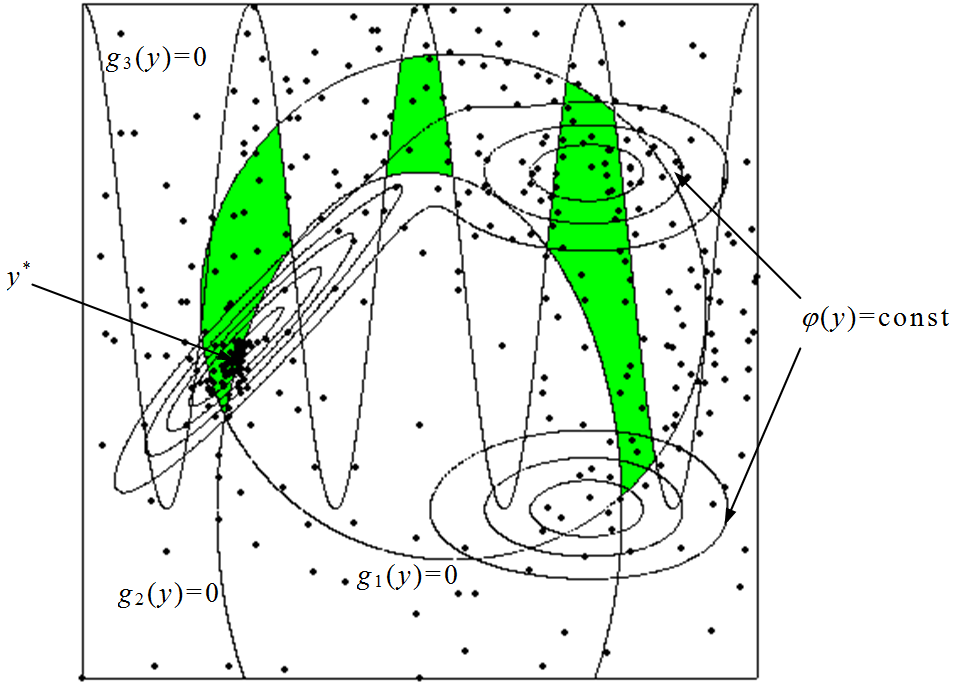
\includegraphics[width=0.8\linewidth]{figures/6_8.png}
\caption{The results of solving the problem using six processors}
\label{6_fig_8}     
\end{figure}
\end{example}

The results of the experiments (the number $k_i$ of computations of the values of the problem functions $g_i(y)$) are presented in tables \ref{6_tab2}--\ref{6_tab4}. Table~\ref{6_tab1} corresponding to the sequential algorithm is presented for comparison. 

\begin{table}
	\caption{The results of solving the problem on single processor}
	\label{6_tab1}
	\center
	\begin{tabular}{ccccc}
		\hline\noalign{\smallskip}
		$l$  & $k_1$ & $k_2$ & $k_3$ & $k_4$    \\
		\noalign{\smallskip} \hline \noalign{\smallskip}
		1 	&	1098 &	623 & 392	& 152 \\
		\noalign{\smallskip}\hline
	\end{tabular}
\end{table}

\begin{table}
	\caption{The results of solving the problem on two processors}
	\label{6_tab2}
	\center
	\begin{tabular}{cccccc}
		\hline\noalign{\smallskip}
		$l$  & $k_0$ &$k_1$ & $k_2$ & $k_3$ & $k_4$    \\
		\noalign{\smallskip} \hline \noalign{\smallskip}
		1 	&	636 &	567 & 331	& 212 & 104 \\
		2 	&	632 &	327 & 193	& 125 & 61 \\
		\noalign{\smallskip}\hline\noalign{\smallskip}
		Total 	&	1268 &	894 & 524	& 337 & 165 \\
		\noalign{\smallskip}\hline
	\end{tabular}
\end{table}

\begin{table}
	\caption{The results of solving the problem on four processors}
	\label{6_tab3}
	\center
	\begin{tabular}{cccccc}
		\hline\noalign{\smallskip}
		$l$  & $k_0$ &$k_1$ & $k_2$ & $k_3$ & $k_4$    \\
		\noalign{\smallskip} \hline \noalign{\smallskip}
1	&	585	&	508	&	311	&	206	&	88	\\
2	&	579	&	262	&	157	&	86	&	36	\\
3	&	579	&	293	&	174	&	119	&	41	\\
4	&	579	&	284	&	178	&	116	&	48	\\
		\noalign{\smallskip}\hline\noalign{\smallskip}
		Total	&	2322	&	1347	&	820	&	527	&	213 \\
		\noalign{\smallskip}\hline
	\end{tabular}
\end{table}

\begin{table}
	\caption{The results of solving the problem on six processors}
	\label{6_tab4}
	\center
	\begin{tabular}{cccccc}
		\hline\noalign{\smallskip}
		$l$  & $k_0$ &$k_1$ & $k_2$ & $k_3$ & $k_4$    \\
		\noalign{\smallskip} \hline \noalign{\smallskip}
1	&	354	&	289	&	165	&	105	&	44	\\
2	&	346	&	90	&	55	&	28	&	10	\\
3	&	346	&	113	&	66	&	40	&	10	\\
4	&	346	&	160	&	87	&	48	&	25	\\
5	&	346	&	224	&	119	&	68	&	23	\\
6	&	346	&	274	&	159	&	97	&	37	\\
		\noalign{\smallskip}\hline\noalign{\smallskip}
Total	&	2084	&	1150	&	651	&	386	&	149	\\
		\noalign{\smallskip}\hline
	\end{tabular}
\end{table}


The iteration speedup of the parallel algorithm on $p$ processors is presented in Table~\ref{6_tab5}. The iteration speedup was defined as the ratio of the number of iteration (which is equal to the number of checks of the first constraint $g_1$) executed by the sequential algorithm to the maximum number of iterations executed by the parallel algorithm on one of processors. This method of determining the speedup is important for the problems, in which the estimates of the functions' values requires considerable computational costs.

\begin{table}
	\caption{Iteration speedup of the parallel algorithm }
	\label{6_tab5}
	\center
	\begin{tabular}{cc}
		\hline\noalign{\smallskip}
		$p$  & speedup     \\
		\noalign{\smallskip} \hline \noalign{\smallskip}
		1 	&	--- \\
		2 	&	1.93 \\
		4 	&	2.16 \\
		6 	&	3.8 \\
		\noalign{\smallskip}\hline
	\end{tabular}
\end{table}

The results of the experiments clearly demonstrate the effect of speed up (the reduction in the number of the costly computations of the problem functions).

\section{Parallel computations based of novel schemes for building the multiple Peano curves}
\subsection{Scheme for building the rotated evolvents}

The application of the scheme for building the multiple evolvents (hereinafter called the shifted evolvents or $S$-evolvents) described in Subsection \ref{6_section_shift} allows to preserve the information on the nearness of the points in the multidimensional space and, therefore, to provide more precise (as compared to a single evolvent) estimate of Lipschitz constant in the search process. However, this approach has serious restrictions, which narrow the applicability of the parallel algorithms, designed on the base of the $S$-evolvents.

Because a shifted evolvent is built as a result of the shift of a hypercube $D$ along the main diagonal, and the shift step decreases 2 times for the building of each subsequent mapping, the number of such shifts is limited by the evolvent density $m$. In the case when the shift step is less than $2^{-m}$, the next evolvent coincides with the previous one. Thus, the applicable number of the evolvents $L$ and, hence, the number of processors are limited by $m$ ($L\leq m$), where $m$ is the density of the evolvents.

Also, it follows from the algorithm for building the shifted evolvents that solving the initial problem in the domain $D$ is reduced to solving a set of problems in the extended domains $D_l$ from (\ref{6_hypercubes}) with additional constraint (\ref{6_g0}). As a result, the structure of the search domain becomes more complicated, and the exponential decrease of the volume of the search domain $D$ in relation to the volumes of the domains $D_l$ with increasing dimensionality of the problem takes place.

To overcome the disadvantages mentioned above and to preserve the information on the nearness of the points in the $N$-dimensional space, a novel scheme of building of the multiple mappings is proposed. The building of a set of Peano curves not by the shift along the main diagonal of the hypercube but by rotation of the evolvents around the coordinate origin is a distinctive feature of the proposed scheme \cite{6_Gergel2009}. In the initial non-rotated mapping for close points $y', y''$ in the multidimensional space their preimages  $x', x''$ in the interval $[0,1]$ can be far away from each other. In the rotated scheme there exists a mapping $y^i(x)$ according to which preimages $x', x''$ will be located nearer. The evolvents generated according to the novel scheme will be hereinafter called the rotated evolvents or $R$-evolvents.

In Fig.~\ref{6_fig_9} two evolvents being the approximations to Peano curves for the case $N=2$ are presented as an illustration. The grid nodes in the $N$-dimensional space are marked by the dark dots. A pair of points, the preimages of which are far away from each other on the one-dimensional axis for one mapping and are close to each other for another mapping is pointed by the arrows. The maximum number of various rotations of the evolvents mapping the $N$-dimensional hypercube onto a one-dimensional interval is $2^N$. The employment of all possible rotations might appear to be redundant. In this case, one can select only a part of all rotations.

\begin{figure}[t]
%\sidecaption[t]
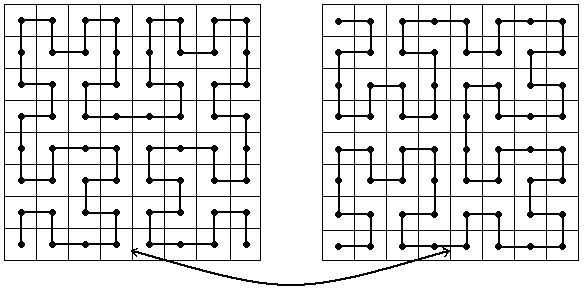
\includegraphics[width=0.8\linewidth]{figures/6_9.png}
\caption{Close/far points for the rotated evolvents}
\label{6_fig_9}     
\end{figure}

As a possible approach, one can propose to generate the new evolvents by the rotation of the initial evolvents on the angle of $\pm\pi/2$ in each of the coordinate planes. For example, the rotation matrices in the plane $(y_2,y_4)$ for  $N=5$ are presented below.
\begin{eqnarray*} 
 \begin{pmatrix}
  1 & 0 & 0 & 0 & 0 \\
  0 & 0 & 0 & -1 & 0 \\
  0 & 0 & 1 & 0 & 0 \\
  0 & 1 & 0 & 0 & 0 \\
  0 & 0 & 0 & 0 & 1
 \end{pmatrix}
\qquad \qquad
 \begin{pmatrix}
  1 & 0 & 0 & 0 & 0 \\
  0 & 0 & 0 & 1 & 0 \\
  0 & 0 & 1 & 0 & 0 \\
  0 & -1 & 0 & 0 & 0 \\
  0 & 0 & 0 & 0 & 1
 \end{pmatrix}
\end{eqnarray*} 

The number of such pairs of rotations is determined by the number of the coordinate planes in the space, which equals to  $N(N-1)/2$. The total number of the transformations equals to $N(N-1)$. Taking into account the initial mapping, one can conclude that this method allows to build up to $N(N-1)+1$ evolvents for mapping the $N$-dimensional domain onto the corresponding one-dimensional intervals. Moreover, the additional constraint  $g_0(y) \leq 0$ with $g_0(y)$ from (\ref{6_g0}), which arises in shifted evolvents, is absent. This method for building a set of mappings can be ``scaled'' easily to obtain more evolvents (up to $2^N$) if necessary.

The use of the set of mappings $Y_L(x)=\{y^1(x),...,y^L(x)\}$ results in the appearing of the corresponding set of the one-dimensional multiextremal problems 
\begin{equation}\label{6_problem_lr} 
\min{\left\{\varphi(y^l(x)):x\in [0,1], \; g_j(y^l(x))\leq 0, \; 1 \leq j \leq m\right\}}, \ 1 \leq l \leq L.
\end{equation} 
Each problem from this set can be solved independently. Any computation of the value $z=g_\nu(y'),\ y'=y^i(x')$ of the function $g_\nu(y)$ in the $i$-th problem can be interpreted as a computation of the value $z=g_\nu(y'),\ y'=y^s(x'')$ for any other $s$-th problem without time-comsuming computations of the functions $g_\nu(y)$. Such information integrity allows to solve  initial problem (\ref{6_problem}) by solving $L$ problems (\ref{6_problem_lr}) on a set of intervals $[0,1]$ in parallel by the index method. 

The decision rules for the parallel algorithm using $R$-evolvents coincide with the ones of the sequential algorithm almost completely except the method of the trial execution. Namely, the execution of a trial at the point $x^k \in [0,1]$ in the $s$-th problem in the case of using $R$-evolvents consists in the following sequence of operations.

\begin{enumerate}
	\item Determine the image $y^k=y^s(x^k)$ according to the mapping  $y^s(x)$.
	\item Inform the rest processors on the beginning of the trial execution at the point  $y^k$ (\textit{the blocking} of the point $y^k$).
	\item Compute the values $g_1(y^k),...,g_\nu(y^k),$ where the index $\nu \leq m$ are determined by the conditions
	\[
	g_j(y^k)\leq 0,\ 1\leq j< \nu,\ g_\nu(y^k) > 0,\ \nu \leq m.
	\]
	The first violation of the constraints terminates the trial at the point  $y^k$. In the case when $y^k$ is a feasible one, the trial includes the computation of all functions of the problem, and the index value is set to $\nu = m+1$. The triplet
	\begin{equation}\label{6_triplet_r} 
	y^s(x^k),\ \nu = \nu(x^k),\ z^k=g_\nu(y^s(x^k))
	\end{equation}
	is  \textit{the trial result} at the point $x^k$.
	\item Determine the preimages $x^{kl} \in [0,1],\; 1\leq l \leq L,$ of the point $y^k$ and interpret the trial executed at the point $y^k \in D$ as the execution of the trials in the $L$ points 
	\[
	x^{k1},...,\ x^{kL}
	\]
	with the same result 
	\[
	\nu(x^{k1})=...=\nu(x^{kL})=\nu(x^k),	
	\]
	\[
	g_\nu(y^1(x^{k1}))=...=g_\nu(y^L(x^{kL}))=z^k	
	\]
	and inform the rest processors on the results of the trial at the point $y^k$.		
\end{enumerate}

\subsection{Comparison of the algorithms}

\begin{example}

In order to compare the efficiency of the algorithms, the method of the operation characteristics has been applied. The series of experiments was devoted to minimixation of 100 two-dimensional functions of two variables
\begin{eqnarray} \label{6_VAG}
\varphi(y)= -&\left\{\left(\sum^{7}_{i=1}\sum^{7}_{j=1}A_{ij}g_{ij}(y)+B_{ij}h_{ij}(y)\right)^2+\right. \\
&\left.\left(\sum^{7}_{i=1}\sum^{7}_{j=1}C_{ij}g_{ij}(y)+D_{ij}h_{ij}(y)\right)^2\right\}^{1/2},\\ \nonumber
\end{eqnarray}
where
\begin{eqnarray} \nonumber
& y=(y_1,y_2)\in R^2, 0 \leq y_1,y_2 \leq 1, \\ \nonumber
& g_{ij}(y)=\sin(i\pi y_1)\sin(j\pi y_2),  \\ \nonumber
& h_{ij}(y)=\cos(i\pi y_1)\cos(j\pi y_2), \nonumber 
\end{eqnarray}
and coefficients $A_{ij}, B_{ij}, C_{ij}, D_{ij}$  are taken uniformly in the interval $[-1,1]$.

The experiments have been carried out for the algorithms described above with $S$-evolvents and $R$-evolvents  with the density $m = 12$. The number of evolvents $L = 2$, the parameters $r=2.1,\ \epsilon = 0.01$ and the reserves $\epsilon_\nu= 0.05$ from (\ref{6_z_nu}) have been used. These parameters are the minimal ones for the corresponding methods, for which the $100\%$ of the problems was solved. 

The operation characteristics of the methods obtained for the problem series generated according to (\ref{6_VAG}) are presented in Fig.~\ref{6_fig_11}. The lower dashed curve corresponds to the shifted evolvents method, the middle dashed one corresponds to the method with a single evolvent, and the upper solid curve corresponds to the rotated evolvents method. Such position of the curves demonstrates that the algorithm with $R$-evolvents provides in average faster obtaining the trial points falling into the predefined vicinity of the solution than the algorithm with $S$-evolvents  or the algorithm with a single evolvent.

\begin{figure}[t]
%\sidecaption[t]
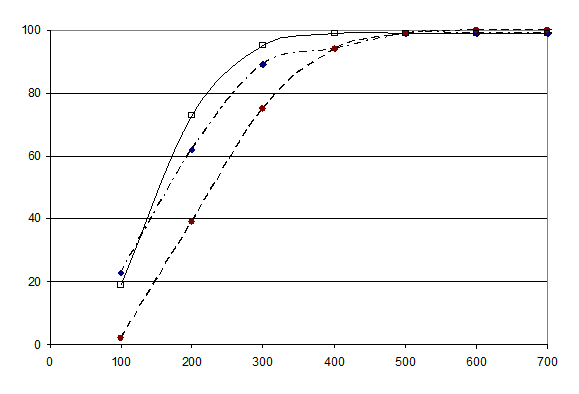
\includegraphics[width=0.8\linewidth]{figures/6_11.png}
\caption{The operation characteristics}
\label{6_fig_11}     
\end{figure}

\end{example}

\begin{example}
To illustrate the work of the parallel algorithm with $R$-evolvents for solving the essentially multidimensional problems, let us consider the minimization problem of the function
\[
\varphi(y) = \sum_{i=1}^N{\left(y_i^2-cos(18y_i^2)\right)},\ -1.5\leq y_i\leq 1.5, \ 1\leq i\leq N,\ N=6,
\]
where the minimum value $\varphi(y^\ast) = -N$ is achieved at the point $y^*=0$.

To solve this problem, the sequential method and the parallel one with the rotated evolvents with the density $m = 10$ were used. The parameter of the method $r=2.0$ and accuracy $\epsilon = 0.05$ in the termination criterion were employed. The number of evolvents $L = 30$ corresponds to the number of processors involved in solving the problem. The sequential algorithm as well as the parallel one have found the solution with the required precision; the sequential algorithm has executed 173116 iterations while the parallel one has executed 8535 (the maximum number of iterations for one processor). The iteration speedup was 20.28 and the time speedup was 7.48.
\end{example}

\begin{example}
Let us consider now the problem of minimization of the function from the previous example in the domain  $-1\leq y_i \leq 1,\ 1\leq i\leq N,$ for $N=15, 20$. In this experiment 100 processors were used. The speedup in time and the efficiency of finding the global optimum with respect to the number of trials with equal termination conditions were estimated. The results of solving the problems are presented in Table~\ref{6_tab_l1}.
	
	\begin{table}
	\caption{The results of multidimensional functions minimization}
	\label{6_tab_l1}
	\center
	\begin{tabular}{cccccccc}
		\hline\noalign{\smallskip}
		$N$ & $k$ & \multicolumn{2}{c}{ Sequential algorithm  } &\ & \multicolumn{3}{c}{Parallel algorithm } \\
		\noalign{\smallskip} \cline{3-4} \cline{6-8} \noalign{\smallskip}
		 & & Time & $\varphi_k^\ast$  &\  & Time & $\varphi_k^\ast$ & Speedup  \\
		\noalign{\smallskip} \hline \noalign{\smallskip}
%		11	&	$5\cdot10^6$	&	544068.8 & $-10.997$	& &	9321.5 & $-10.995$ 	&	112.01	\\
		15\	&	$3\cdot10^6$ \ &	605788 & $-14.835$	& &	7414 & $-14.925$ 	&	81.7	\\
		20\	&	$3\cdot10^6$ \ &	605956 & $-19.989$	& &	6654 & $-19.048$ 	&	91.06	\\
		\noalign{\smallskip}\hline
	\end{tabular}
\end{table}

It is clear from Table~\ref{6_tab_l1} that the index method with $R$-evolvents executed on 100 processors demonstrated the speedup close to the linear one with respect to the computational time that gives evidence its high efficiency.
\end{example}
\begin{example}
Now let us demonstrate the efficiency of the parallel index method in solving the constrained global optimization problem
\[
\varphi(y) = N + \sum_{i=1}^N{\left(y_i^2-\cos(2\pi y_i)\right)}\rightarrow\min 
\]
\[
g_1(y) = \sum_{i=1}^N{y_i} - 0.5 \leq 0
\]
\[
g_2(y) = \sum_{i=1}^N{y_i^2} - 1.0 \leq 0
\]
\[
g_3(y) = \sum_{i=1}^N{\sin(i\pi y_i)} - 0.3 \leq 0
\]
for $-1\leq y_i\leq 1,\ 1\leq i\leq N,\ N=8$. The results of solving this problem by the sequential method and by the parallel method on 56 processors are presented in Table~\ref{6_tab_l2}. In both cases, the methods terminated the search process upon achievement the predefined accuracy $\epsilon = 0.0035$. Table~\ref{6_tab_l2} shows number of trials $k$, number of objective function evaluations $k_4$, time of comutations $t$ in seconds, speedup in time $s$, iterations $S$ and in objective function evaluations $S_4$.
The maximum number of trials and objective function evaluations per one processor is specified in brackets.

	\begin{table}
	\caption{Comparison of the algorithms in solving a constrained problem}
	\label{6_tab_l2}
	\center
	\begin{tabular}{cccccccc}
		\hline\noalign{\smallskip}
		 Method & $k$ & $k_4$ & $S$ & $S_4$ & $t$ & $s$ & $\varphi_k^\ast$  \\
		\noalign{\smallskip} \hline \noalign{\smallskip}
		Sequential	&	309640 &	33874 & ---	& --- &	40006 & ---	&	0.016	\\
		Parallel	&	244356 (4891) \ &	22722 (789) & 63.3	& 42.9 &	626 & 63.8 	&	0.022	\\
		\noalign{\smallskip}\hline
	\end{tabular}
\end{table}

It is evident from Table~\ref{6_tab_l2} that the parallel algorithm demonstrated the speed up 63.3 with respect to the number of trials, 42.9 with respect to the number of objective function computations, and of 63.8 with respect to the computation time.
Note that the comparison of the sequential algorithm with the parallel one appears to be more difficult in the problems of higher dimensionality since in the latter case all the search information is concentrated in one computational node. There appeared to be not enough RAM for the sequential algorithm run on a single node. As a result, the swapping was activated. In the parallel algorithm, all data are distributed among the processors. This allows not to use the external memory for storing the search information.

\end{example}

\begin{thebibliography}{99.}

\bibitem{6_Sergeyev2006}
Sergeyev, Ya.D., Kvasov, D.E.: Global search based on efficient diagonal partitions and a set of Lipschitz constants. SIAM J. Optim. \textbf{16(3)}, 910--937 (2006)

\bibitem{6_Sergeyev2015}
Sergeyev, Ya.D., Kvasov, D.E.: A deterministic global optimization using smooth diagonal auxiliary functions. Communications in Nonlinear Science and Numerical Simulation. \textbf{21}, 99--111 (2015)

\bibitem{6_Sergeyev2017}
Sergeyev, Ya.D., Kvasov, D.E.: Deterministic global optimization: An introduction to the diagonal approach. Springer, New York (2017)

\bibitem{6_Zilinskas2008}
\v{Z}ilinskas, J.: Branch and bound with simplicial partitions for global optimization. Mathematical Modelling and Analysis \textbf{13(1)}, 145--159 (2008)

\bibitem{6_Zilinskas2014}
Paulavi\v{c}ius, R., \v{Z}ilinskas, J.: Simplicial Lipschitz optimization without the Lipschitz constant. J. Glob. Optim. \textbf{59(1)}, 23--40  (2014)

\bibitem{6_Zilinskas2014_1}
Paulavi\v{c}ius, R., \v{Z}ilinskas, J.: Simplicial Global Optimization. SpringerBriefs in Optimization, Springer, New York (2014)

\bibitem{6_Strongin2000}
Strongin, R.G., Sergeyev, Ya.D.: Global optimization with non-convex constraints. Sequential and parallel algorithms. Kluwer Academic Publishers, Dordrecht (2000)

\bibitem{6_Strongin2013}
Sergeyev, Ya.D., Strongin, R.G., Lera, D.: Introduction to Global Optimization Exploiting Space-Filling Curves. SpringerBriefs in Optimization, Springer, New York (2013)

\bibitem{6_Gourdin}
Gourdin, E., Jaumard, B., Ellaia, R.: Global optimization of H\"{o}lder functions. J. Global Optim. \textbf{8}, 323--348 (1996)

\bibitem{6_Lera2002}
Lera, D., Sergeyev, Y.D.: Global minimization algorithms for H\"{o}lder functions. BIT \textbf{42(1)}, 119--133 (2002)

\bibitem{6_Lera2010}
Lera, D., Sergeyev, Y.D.: Lipschitz and H\"{o}lder global optimization using space-filling curves. Appl. Numer. Math. 60(1–2), 115–129 (2010)

\bibitem{6_Hime}
e Oliveira, H.A., Petraglia, A.: Global optimization using space-filling curves and measure-preserving transformations. Soft Computing in Industrial Applications. \textbf{96}, 121--130 (2011)

\bibitem{6_Lera2015}
Lera, D., Sergeyev, Y.: Deterministic global optimization using space-filling curves and multiple estimates of Lipschitz and Hölder constants. Commun. Nonlinear Sci. Numer. Simul. \textbf{23}, 328--342 (2015)

\bibitem{6_Butz}
Butz, A.R.: Space filling curves and mathematical programming. Inform. Control \textbf{12(4)}, 314--330 (1968)

\bibitem{6_Sagan}
Sagan, H.: Space–Filling Curves. Springer–Verlag, New York (1994)

\bibitem{6_Strongin1991}
Strongin, R.G.: Parallel multi-extremal optimization using a set of evolvents. Comp. Math. Math. Phys. \textbf{31(8)}, 37--46 (1991)

\bibitem{6_Strongin1992}
Strongin, R.G.: Algorithms for multi-extremal mathematical programming problems employing the set of joint space-filling curves. J. Global Optim. \textbf{2(4)}, 357--378 (1992)

\bibitem{6_Gergel2009}
Strongin, R.G., Gergel, V.P., Barkalov, K.A.: Parallel methods for global optimization problem solving. Journal of instrument engineering. \textbf{52}, 25--33 (2009) (In Russian)

\end{thebibliography}

%\end{document}
